\section{Introducción}
En este capítulo describiré el conjunto de datos de la lista de problemas, cómo ha sido su distribución en el tiempo y seleccionaré algunos elementos del contexto: (a) área jerárquica del especialista, (b) grupo etario del paciente y (c) nivel de asistencia, para evaluar en el siguiente capítulo si inciden en los problemas médicos que son registrados. 

También describo los procesos de ETL que realicé para que los experimentos fuesen comparables con los realizados en otras instituciones.

El proceso más complejo fue la reducción de la cardinalidad de las áreas jerárquicas, que pasaron de ser 918 a 29 servicios de atención de salud mapeados a servicios de SNOMED CT. Los conceptos que se agrupan alrededor de estos servicios de atención son llamados \textit{refsets} por especialidad médica y fueron creados con el histórico de la lista de problemas.

Uno de los aspectos claves en el uso significativo de la terminología es la creación de \textit{refsets} que puedan ser utilizados como vocabularios controlados dependientes de contextos. Estos \textit{refsets} facilitan el uso de SNOMED CT como terminología de codificación primaria para la lista de problemas u otros niveles de documentación clínica, y maximizaran potencialmente la interoperabilidad de datos a través de las instituciones\cite{Dolin2004KaiserTerminology.}.

Para la construcción de estos \textit{refsets} se siguen dos metodologías, determinar por extensión cuáles son los conceptos que los componen, ya que no es fácil realizar la restricción por una jerarquía o partes de ella \cite{Hjen2014MethodsSets.,Lee2013AImplementations.}; o la generación automática y el uso de \textit{refsets} públicos para comparar el cubrimiento de su contenido \cite{Lee2013AImplementations.}. Este tesis usa la segunda metodología y evalúa el cubrimiento con Kaiser Permanente CMT.

\section{Comprensión de datos}
La lista de problemas registra las observaciones y hallazgos realizados a los pacientes y otra informacion del contexto. Los problemas de los pacientes son descripciones que se agrupan en conceptos, y los conceptos a su vez pertenecen a uno o varios \textit{refsets}.
Cuando se registra un problema, se asocia el área jerárquica del usuario que ingresó el problema.

El conjunto de datos además tiene el atributo nivel de asistencia que indica el ámbito en el que fue cargado el problema (1 = Ambulatorio , 2 = Internacion General, 3 = Guardia, 4 = Triage, 5 = Internacion Geriatrica, 6 = Internacion Domiciliaria, 7 = Seguimiento Domiciliario, 8 = Episodio Externo, 9 = Episodio Ambulatorio). La figura \ref{fig:ModeloER} contiene el modelo entidad relación, donde se muestra cómo se relacionan estos datos.

\begin{figure}[ht]
\caption{Modelo Entidad-Relación de lista de problemas}
\label{fig:ModeloER}
\centering
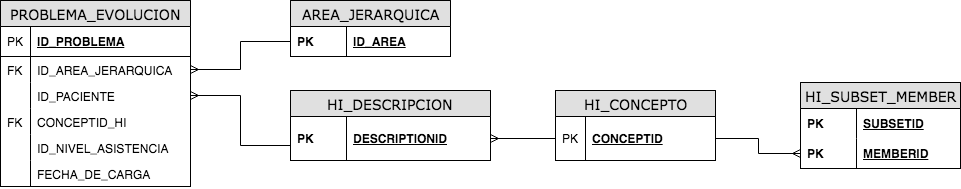
\includegraphics[width=0.9\textwidth]{ER_Problemas}
\end{figure}

\subsection{Distribución en el tiempo}
El atributo FECHA\_DE\_CARGA indica la fecha en la que se cargó el problema por primera vez, las posteriores veces se vuelve a usar el problema registrado y no se crea uno nuevo. En la figura \ref{fig:registrosYConceptos}, se puede observar que aunque la implementación de la HCE empezó en el año 1998, hay registros anteriores a esa fecha los cuales se interpretan como errores en el momento de la carga, al igual que los registros con las fechas superiores al 2017. En total son \num{9149} casos que corresponden al \num{0,004}\% de los datos.

Como se muestra en la figura \ref{fig:registrosYConceptos} la distribución no es uniforme, su crecimiento se explica por los hitos de implementación dentro de la HC, en el año \num{2002} se generalizó el uso de la HCE en todo el hospital, y en el año \num{2006} se implementó el servidor de terminología. Los años \num{2015} y \num{2016} muestran un incremento en el registro de la lista de problemas.

En cuanto a los conceptos diferentes registrados por año, se observa una distribución más uniforme, especialmente después del año \num{2007}.Los datos del año 2017 son sólo los del primer semestre.

\begin{figure}[ht]
\caption{Distribución de problemas por año de carga}
\label{fig:registrosYConceptos}
\centering
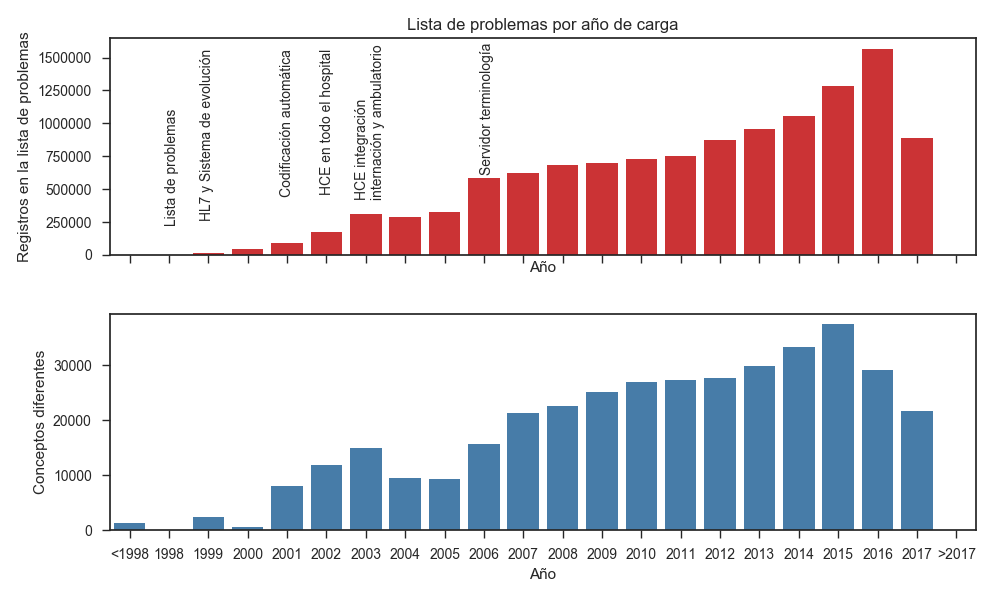
\includegraphics[width=\textwidth]{chart1}
\end{figure}

\subsection{Distribución por individuo}
Según la figura \ref{fig:listaIndividuos} la mayoría de los individuos tiene sólo un problema registrado en su lista de problemas, estos corresponde al \num{34.1}\% de los datos. Los individuos que tienen registrados hasta 10 problemas en la lista son el \num{80}\% de los datos.

\begin{figure}[ht]
\caption{Distribución del tamaño de la lista de problemas por individuos}
\label{fig:listaIndividuos}
\centering
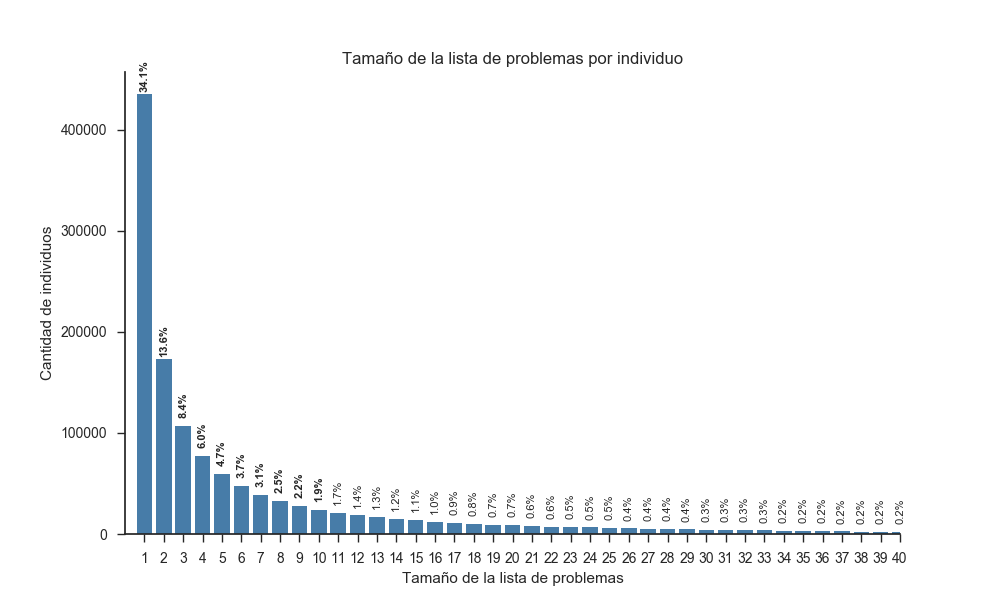
\includegraphics[width=\textwidth]{chart2}
\end{figure}

\subsection{Distribución por conceptos}
El conjunto de datos contiene \num{88869} conceptos distintos usados para identificar problemas de los pacientes. La figura \ref{fig:listaProblemas} representa el uso de estos conceptos dentro de la RMOP, en ella puedo observar que un conjunto pequeño de problemas tiene una frecuencia muy alta y el resto que queda en la cola de la distribución son usados muy pocas veces. Los conceptos más frecuentemente usados son Control de salud, Fiebre, Dolor abdominal,  Hipertensión arterial, Catarro de las vías áreas superiores, Malestar general, Tos, Embarazo, Lumbalgia, Broncoespasmo, Evaluación inicial del paciente e Infección del tracto urinario, que juntos son el \num{20}\% del total de registros. 

El desafío de esta tesis es investigar si hay conceptos que estén correlacionados entre si, que puedan ser útiles para ser sugeridos como parte de la lista de problemas de los pacientes dentro de determinados contextos. 

\begin{figure}[ht]
\caption{Distribución de todos los problema por su aparición en la lista}
\label{fig:listaProblemas}
\centering
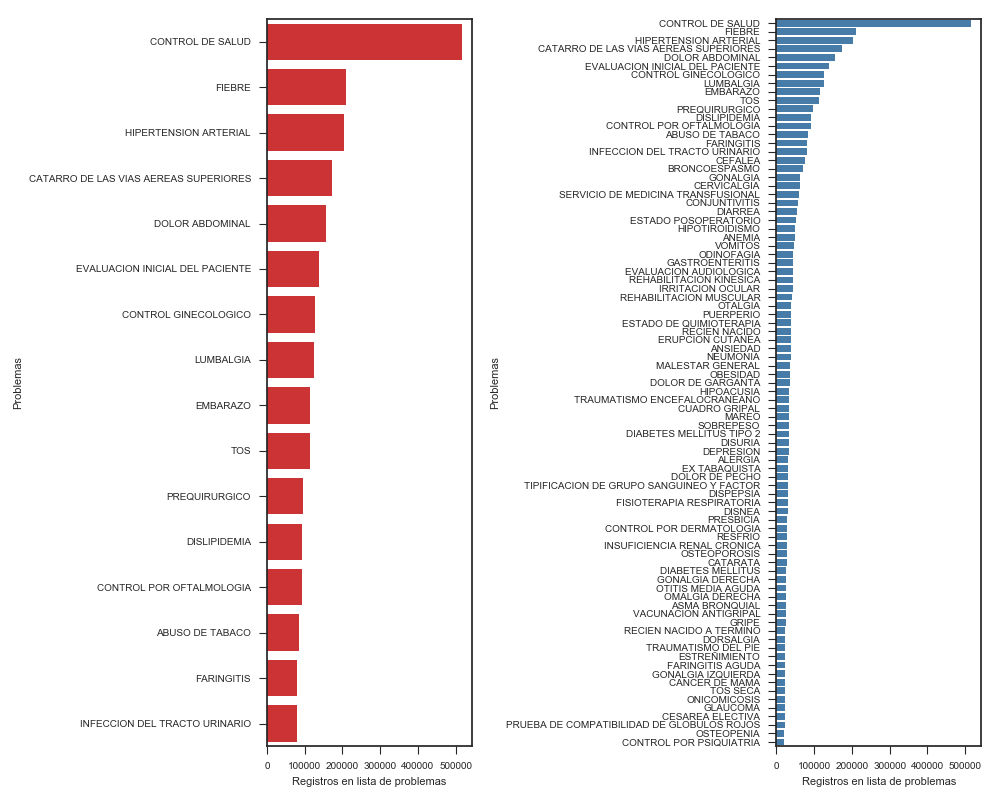
\includegraphics[width=\textwidth]{chart3}
\end{figure}

\subsection{Distribución por contextos}
Los contextos que tuve en cuenta en esta tesis fueron área jerárquica, nivel de asistencia y grupo etario, a continuación describo cómo se distribuyen los conceptos y registros de la RMOP en los contextos.


\subsubsection{Contexto: Área Jerárquica}
La HCE tiene 918 áreas jerárquicas, de las cuales 601 tienen usuarios que han registraron problemas dentro de la lista de algún paciente. Hay dos jerarquías que usan más de \num{20000} conceptos (Clínica médica y Medicina Familiar), el resto de jerarquías usan en promedio menos de 5000 conceptos. 

Las áreas jerárquicas que tiene el HIBA responden a necesidades operativas de la HCE, pero su nivel de disgregación no significa que la lista de problemas necesite también ese nivel de detalle, por el contrario se evidencia al aplicar algoritmos de agrupamiento que hay solapamientos de jerarquías. Con el objetivo de reducir la cardinalidad en las áreas jerárquicas y agruparlas dentro de las más representativas e interoperables, seguí la metodología que se encuentra en la figura \ref{fig:MetodologiaReduccionAreas}.


\begin{figure}[ht]
\caption{Metodología para reducción de áreas jerárquicas}
\label{fig:MetodologiaReduccionAreas}
\centering
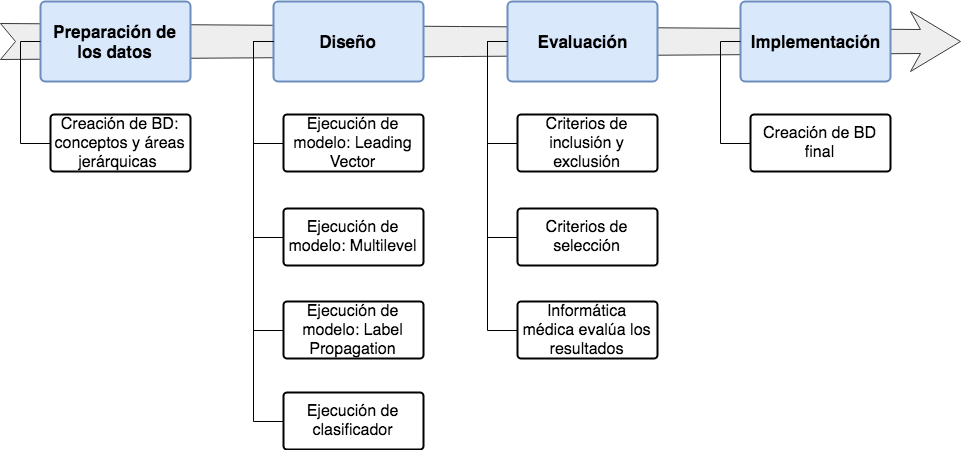
\includegraphics[width=0.9\textwidth]{Reducci_n_cardinalidad}
\end{figure}

En la primera fase de preparación de los datos, cree la base de datos de grafos. En el modelo de datos que se observa en la figura \ref{fig:ModeloDatosAreas} los nodos son los conceptos y las áreas jerárquicas, y las relaciones son las jerarquías (ES\_UN) entre los conceptos y su uso (REGISTRA\_PROBLEMA)  por el área. De tal manera que se represente los diferentes niveles de generalización de los conceptos con la relación (ES\_UN), y que un área jerárquica tiene varios conceptos y un concepto puede estar en varias áreas con la relación (REGISTRA\_PROBLEMA). 

\begin{figure}[ht]
\caption{Modelo de datos}
\label{fig:ModeloDatosAreas}
\centering
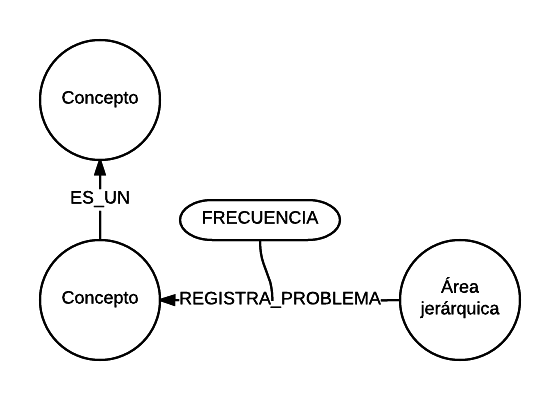
\includegraphics[width=0.5\textwidth]{Modelo_grafo_areas}
\end{figure}

La segunda fase tiene el propósito de encontrar qué áreas jerárquicas comparten similares conceptos, y así identificar las áreas que se pueden agrupar como una sola. En el segundo experimento el propósito es identificar los servicios que se están solapando entre sí, usé un algoritmo de aprendizaje supervisado para predecir el servicio al que pertenecen los conceptos, este algoritmo tiene mayor dificultad para predecir el servicio si hay muchos conceptos similares entre ellos por lo tanto serían candidatos a fusión.

La tercera fase es para evaluar el modelo, se compone de:(a) Informáticos médicos determinan si los criterios se deben aplicar a cada una de las 918 áreas, y (b) Evaluación de la cobertura de los \textit{refsets} formados a partir de los servicios finales.

\paragraph{Fase de diseño:Experimento 1 (Agrupamiento de áreas jerárquicas)}

\subparagraph{Criterios de exclusión}

\begin{itemize}
\item Áreas jerárquicas con sólo un concepto seleccionado.
\item Áreas jerárquicas dentro del cluster de administrativos, las cuales corresponden a usuarios que seleccionaron problemas por razones operativas administrativas y no por razones médicas.
\end{itemize}

\subparagraph{Criterios de selección}
\begin{itemize}
\item Los servicios de la atención de la salud de la jerarquía de SNOMED CT son usados para mapear los del HIBA, de tal manera que los servicios finales permitan la interoperabilidad con otros centros de salud. Para realizar el mapeo, hice una búsqueda en SNOMED CT con string matching del nombre del área del HIBA o del área más general que la contenía.
\item Si no hay un mapeo, seleccioné el servicio de las áreas que están dentro del mismo cluster de label propagation y multilevel, y que además hayan seleccionado los mismos conceptos.
%\item Si al aplicar un algoritmo de clasificación se presenta un alto solapamiento de conceptos entre servicios, estos son candidatos a fusionarse
\end{itemize}

\subparagraph{Diseño del modelo}: Ejecuté 3 algoritmos de agrupamiento. como se observa en la tabla \ref{clusteringAreas}, el algoritmo leading vector dividió el conjunto de datos en 2 y su modularidad es la más baja por lo tanto sus resultados se descartaron.  Los resultados de los otros dos algoritmos fueron usados en los criterios de selección de jerarquía.

\begin{table}[htb]
\centering
\caption{Agrupamiento de áreas jerárquicas y conceptos}
\label{clusteringAreas}
\begin{tabular}{@{}llll@{}}
\toprule
Algoritmo         & Modularidad & Grupos & Test \\ \midrule
Label Propagation & 0.165       & 18     &      \\
Leading Vector    & 0.144       & 2      &      \\
MultiLevel        & 0.447       & 14     &      \\ \bottomrule
\end{tabular}
\end{table}

\paragraph{Fase de diseño:Experimento 2 (Clasificador de áreas jerárquicas)}

\subparagraph{Criterios de selección}
\begin{itemize}
\item Si al aplicar un algoritmo de clasificación se presenta un alto solapamiento de conceptos entre servicios, estos son candidatos a fusionarse
\end{itemize}

\subparagraph{Diseño del modelo}: 
Un enfoque de clasificación permite identificar aquellos servicios que tienen una superposición de conceptos. Usé el algoritmo de aprendizaje supervisado StanfordNLP ColumnClassifier \cite{manning-EtAl:2014:P14-5},  para predecir el servicio al que pertenecen los conceptos, este algoritmo tiene mayor dificultad al predecir el servicio si hay muchos conceptos similares entre ellos.

\paragraph{Evaluación final del modelo}: Ejemplos de los resultados de la aplicación de los criterios de exclusión y de selección del primer experimento se encuentran en la tabla \ref{ejemploCriterios}. Los resultados de la aceptación de estos criterios se encuentran en la tabla \ref{resultadosCriterios}, el \num{63}\% de los casos fueron excluidos correctamente. Con respecto a los criterios de selección, el \num{96}\% de los casos fueron seleccionados correctamente según la evaluación realizada por la residencia médica.

% Please add the following required packages to your document preamble:
% \usepackage{booktabs}
\begin{table}[htb]
\centering
\caption{Ejemplos de criterios de exclusión y selección}
\label{ejemploCriterios}
\begin{tabularx}{\textwidth}{@{}XlXX@{}}
\toprule
Área Jerárquica                                                          & Excluído? & Servicio Seleccionado            & Observaciones                                                     \\ \midrule
Dirección administrativa                                                 & Si        &                                  & Hace Parte Del Cluster De Administrativos                         \\
Coordinación de turnos - departamento de enfermería                      & Si        &                                  & Tiene un sólo concepto seleccionado.                              \\
Servicio de neurocirugía                                                 & No        & Servicio de neurocirugía         & \textit{String Matching} Con un servicio de Snomed CT                      \\
Sección diálisis peritoneal continua ambulatoria- Servicio de nefrología & No        & Servicio de nefrología adultos   & \textit{String Matching} del área más general con un servicio de Snomed CT \\
Rinología plástica                                                       & No        & servicio de otorrinolaringología & Comparte cluster con áreas con los mismos conceptos.              \\ \bottomrule
\end{tabularx}
\end{table}

% Please add the following required packages to your document preamble:
% \usepackage{booktabs}
\begin{table}[htb]
\centering
\caption{Resultados de la aplicación de los criterios de exclusión y selección}
\label{resultadosCriterios}
\begin{tabular}{@{}lll@{}}
\toprule
Criterio                      & Reportados & Aceptados \\ \midrule
Criterio de exclusión         & 223        & 142       \\
Selección por string matching & 291        & 291       \\
Selección por agrupamiento    & 116        & 111       \\ \bottomrule
\end{tabular}
\end{table}

En este primer experimento reemplacé las 601 áreas jerárquicas con 44 servicios de atención médica de SNOMED CT, y eliminé las que entraron en el criterio de exclusión y fueron aceptadas por el residente.

En el segundo experimento, los datos de entrada son los conceptos y los servicios finales del experimento 1. Realizando una partición de 50\% de los datos para crear entrenamiento y 50\% para test, el modelo creado predice a qué servicio pertenecen los conceptos, con los siguientes F1 score:  Accuracy/micro-averaged F1: 0.736, Macro-averaged F1: 0.500.

La matriz de confusión generada por el modelo aporta información sobre qué servicios comparten los mismos conceptos, y propone así una fusión entre ellos. La tabla \ref{serv_aten_hiba} contiene los 44 servicios que fueron mapeados en el experimento 1, y los 29 servicios finales obtenidos a partir del experimento 2. Al crear un nuevo modelo con los mapeos de los servicios del experimento 2, obtengo los siguientes F1 score: Accuracy/micro-averaged F1: 0.775, Macro-averaged F1:0.664

% Please add the following required packages to your document preamble:
% \usepackage{booktabs}
% \usepackage{graphicx}
\begin{table}[htb]
\centering
\caption{Servicios de atención médica del HIBA}
\label{serv_aten_hiba}
\resizebox{\textwidth}{!}{%
\begin{tabular}{@{}lrrlrrl@{}}
\toprule
Servicios Experimento 1 & F1 Score & TP & Servicios Experimento 2 & F1 Score & Solapados & Acción \\ \midrule
servicio de anestesia & 0,048 & 155 & servicio de medicina general & 0,747 & 1595 & Fusionar \\
servicio audiológico & 0,000 & 0 & servicio de otorrinolaringología & 0,675 & 10 & Fusionar \\
servicio de cardiología adultos & 0,672 & 29589 & servicio de cardiología adultos & 0,672 & - & Mantener \\
servicio de cardiología pediátrica & 0,871 & 9531 & servicio de cardiología pediátrica & 0,871 & - & Mantener \\
servicio de cirugía general & 0,598 & 29993 & servicio de cirugía general & 0,598 & - & Mantener \\
servicio de cirugía pediátrica & 0,437 & 3490 & servicio de cirugía pediátrica & 0,437 & - & Mantener \\
servicio de cirugía plástica & 0,664 & 3619 & servicio de cirugía plástica & 0,664 & - & Mantener \\
servicio de cirugía vascular & 0,178 & 406 & servicio de cardiología adultos & 0,672 & 909 & Fusionar \\
servicio de colposcopía & 0,000 & 0 & servicio de ginecoobstetricia & 0,877 & 293 & Fusionar \\
servicio de dermatología & 0,800 & 39370 & servicio de dermatología & 0,800 & - & Mantener \\
servicio de dermatología pediátrica & 0,405 & 2141 & servicio de dermatología & 0,800 & 3240 & Fusionar \\
servicio de endocrinología & 0,687 & 20509 & servicio de endocrinología & 0,687 & - & Mantener \\
servicio de endocrinología pediátrica & 0,518 & 1003 & servicio de endocrinología pediátrica & 0,518 & - & Mantener \\
servicio de enfermería & 0,595 & 5968 & servicio de enfermería & 0,595 & - & Mantener \\
servicio de farmacia & 0,392 & 112 & servicio de medicina general & 0,747 & 186 & Fusionar \\
servicio de fisioterapia & 0,993 & 34731 & servicio de fisioterapia & 0,993 & - & Mantener \\
servicio de fonoaudiología & 0,612 & 7402 & servicio de otorrinolaringología & 0,675 & 6136 & Fusionar \\
servicio de gastroenterología & 0,233 & 2716 & servicio de medicina general & 0,747 & 13836 & Fusionar \\
servicio de gastroenterología pediátrica & 0,000 & 0 & servicio de otorrinolaringología & 0,675 & 1 & Fusionar \\
servicio de ginecoobstetricia & 0,877 & 77215 & servicio de ginecoobstetricia & 0,877 & - & Mantener \\
servicio de hemoterapia & 0,686 & 374 & servicio de hemoterapia & 0,686 & - & Mantener \\
servicio de imagenología & 0,546 & 2198 & servicio de imagenología & 0,546 & - & Mantener \\
servicio de internacion domiciliaria & 0,131 & 15 & servicio de medicina general & 0,747 & 86 & Fusionar \\
servicio de medicina general & 0,747 & 390596 & servicio de medicina general & 0,747 & - & Mantener \\
servicio de nefrología adultos & 0,674 & 6950 & servicio de nefrología adultos & 0,674 & - & Mantener \\
servicio de neonatología & 0,682 & 11659 & servicio de neonatología & 0,682 & - & Mantener \\
servicio de neumología pediátrica & 0,622 & 1712 & servicio de neumología pediátrica & 0,622 & - & Mantener \\
servicio de neurocirugía & 0,400 & 1371 & servicio de neurocirugía & 0,400 & - & Mantener \\
servicio de neurología adultos & 0,432 & 7436 & servicio de neurología adultos & 0,432 & - & Mantener \\
servicio de neuropediatría & 0,566 & 3028 & servicio de neuropediatría & 0,566 & - & Mantener \\
servicio de odontología adultos & 0,900 & 796 & servicio de odontología adultos & 0,900 & - & Mantener \\
servicio de oftalmología adultos & 0,938 & 57983 & servicio de oftalmología adultos & 0,938 & - & Mantener \\
servicio de oncología clinica & 0,105 & 123 & servicio de oncología clinica & 0,105 & - & Mantener \\
servicio de otorrinolaringología & 0,675 & 24418 & servicio de otorrinolaringología & 0,675 & - & Mantener \\
servicio de patología & 0,000 & 0 & servicio de imagenología & 0,546 & 32 & Fusionar \\
servicio de pediatría & 0,243 & 7699 & servicio de pediatría & 0,243 & - & Mantener \\
servicio de psicología & 0,000 & 0 & servicio de psiquiatria & 0,827 & 32 & Fusionar \\
servicio de psiquiatria & 0,827 & 8268 & servicio de psiquiatria & 0,827 & - & Mantener \\
servicio de psiquiatria pediátrica & 0,945 & 4159 & servicio de psiquiatria pediátrica & 0,945 & - & Mantener \\
servicio de reumatología & 0,336 & 96 & servicio de medicina general & 0,747 & 226 & Fusionar \\
servicio de terapia intensiva & 0,275 & 968 & servicio de medicina general & 0,747 & 1725 & Fusionar \\
servicio de terapia intensiva pediátrica & 0,179 & 156 & servicio de medicina general & 0,747 & 308 & Fusionar \\
servicio de traumatología & 0,821 & 143770 & servicio de traumatología & 0,821 & - & Mantener \\
servicio de urología & 0,678 & 15232 & servicio de urología & 0,678 & - & Mantener \\ \bottomrule
\end{tabular}%
}
\end{table}

El último nivel de evaluación lo realicé midiendo el cubrimiento de los servicios\cite{Yu2012ClinicalSNOMED-CT}, el cual está definido como la proporción de los conceptos que se comparten con un servicio, al tamaño del \textit{refset} de referencia, como se define en la ecuación \ref{eq:cubrimiento}
\begin{equation}\label{eq:cubrimiento}
\textup{cubrimiento} = \frac{\textup{conceptos mapeados en T}}{\textup{Tamaño de T}}
\end{equation}

\begin{itemize}
\item \textit{Conceptos mapeados en T}, es el número total de conceptos de Snomed CT que se comparten con el \textit{refset} de referencia $T$, y
\item el \textit{tamaño de T} es el número total de conceptos que tiene el \textit{refset} de referencia $T$.
\end{itemize}

La validación del cubrimiento de los servicios implican la comparación de los mismos con otros que ya estén avalados, para realizar esta comparación usé el conjunto de de términos llamados \textit{Convergent Medical Terminology (CMT) }construído por \textit{Kaiser Permanente}. La tabla \ref{subsetsComparacion} contiene los servicios que se compararon con \textit{CMT}, en algunos casos necesité unir varios servicios para comparar con uno sólo de \textit{CMT} como el caso de los servicios de nefrología de adultos, endocrinología, endocrinología pediátrica y urología que se unieron para comprar con el subset \textit{Endocrine, Nephrology, and Urology} de \textit{CMT}.

% Please add the following required packages to your document preamble:
% \usepackage{booktabs}
\begin{table}[htb]
\centering
\caption{Subsets afines entre de HIBA y CMT}
\label{subsetsComparacion}
\begin{tabularx}{\textwidth}{@{}XXl@{}}
\toprule
Servicio HIBA                                                                                                              & Subset Kaiser Permanente & Abreviatura                         \\ \midrule
servicio de cardiologia adultos +\newline  servicio de cardiologia pediatrica                                                       & Cardiology Problem List. Version 2016          & Cardio  \\
servicio de oftalmologia adultos                                                                                           & Ophthalmology Problem List. Version 2016        & Oftalmo \\
servicio de psiquiatria                                                                                                    & Mental Health Subset. Version 2016          & Psiqui     \\
servicio de oncologia clinica                                                                                              & Hematology and Oncology. Version 2015       & Onco     \\
servicio de nefrologia adultos +\newline  servicio de endocrinologia +\newline  servicio de endocrinologia pediatrica +\newline  servicio de urologia & Endocrine, Nephrology, and Urology. Version 2015  & ENU \\
servicio de ginecoobstetricia                                                                                              & Obstetrics and Gynecology. Version 2015        & Gineco  \\
servicio de neurocirugia + servicio de neuropediatria +\newline  servicio de neurologia adultos                                     & Neurology. Version 2015                & Neuro          \\
servicio de dermatologia                                                                                                   & Skin/Dermatology and Respiratory. Version 2015  &Derma  \\
servicio de pediatria                                                                                                      & Pediatrics. Version 2014                     & Pedia    \\
servicio de traumatologia                                                                                                  & Orthopedics. Version 2014                      & Orto  \\ \bottomrule
\end{tabularx}
\end{table}


La tabla \ref{kaiserPermanenteCubrimiento} muestra el cálculo de la cobertura de los \textit{refset} \textit{CMT} comparándolos con los servicios, se puede observar que las mayores coberturas se encuentran en los conjuntos de datos afines relacionados en la tabla \ref{subsetsComparacion}

% Please add the following required packages to your document preamble:
% \usepackage{booktabs}
% \usepackage{multirow}
\begin{table}[htb]
\centering
\caption{Cubrimiento de Kaiser Permanente en Servicios de HIBA}
\label{kaiserPermanenteCubrimiento}
\resizebox{\textwidth}{!}{%
\begin{tabular}{@{}lllllllllll@{}}
\toprule
\multirow{2}{*}{\textbf{Hiba (número de conceptos)}} & \multicolumn{10}{l}{\textbf{Kaiser permanente (número de conceptos)}}                                                                                                                                                                 \\ \cmidrule(l){2-11} 
                                                     & \textbf{Cardio (880)} & \textbf{Derma(2757)} & \textbf{Gineco(1307)} & \textbf{ENU(1639)} & \textbf{Neuro(1792)} & \textbf{Oftalmo(3285)} & \textbf{Onco(4086)} & \textbf{Pedia(3793)} & \textbf{Psiqui (1163)} & \textbf{Orto(5009)} \\ \cmidrule(r){1-1}
Cardio(9182)                                         & 0,46                  & 0,33                 & 0,11                  & 0,20               & 0,19                 & 0,09                   & 0,14                & 0,34                 & 0,13                   & 0,15                \\
Derma(11622)                                         & 0,14                  & 0,45                 & 0,08                  & 0,11               & 0,10                 & 0,06                   & 0,20                & 0,27                 & 0,08                   & 0,13                \\
Gineco(8319)                                         & 0,15                  & 0,18                 & 0,33                  & 0,16               & 0,09                 & 0,06                   & 0,11                & 0,27                 & 0,10                   & 0,11                \\
ENU(18075)                                           & 0,31                  & 0,42                 & 0,21                  & 0,40               & 0,42                 & 0,17                   & 0,22                & 0,46                 & 0,28                   & 0,24                \\
Neuro(10856)                                         & 0,26                  & 0,31                 & 0,13                  & 0,19               & 0,40                 & 0,16                   & 0,17                & 0,39                 & 0,26                   & 0,21                \\
Oftalmo (4188)                                       & 0,06                  & 0,06                 & 0,02                  & 0,04               & 0,10                 & 0,41                   & 0,03                & 0,16                 & 0,04                   & 0,09                \\
Onco (721)                                           & 0,07                  & 0,03                 & 0,02                  & 0,03               & 0,03                 & 0,00                   & 0,07                & 0,05                 & 0,02                   & 0,01                \\
Pedia (17325)                                        & 0,26                  & 0,31                 & 0,18                  & 0,27               & 0,25                 & 0,18                   & 0,18                & 0,56                 & 0,22                   & 0,28                \\
Psiqui(2373)                                         & 0,07                  & 0,13                 & 0,07                  & 0,06               & 0,08                 & 0,03                   & 0,03                & 0,16                 & 0,30                   & 0,07                \\
Orto(22555)                                          & 0,21                  & 0,37                 & 0,09                  & 0,13               & 0,24                 & 0,05                   & 0,16                & 0,34                 & 0,10                   & 0,42                \\ \bottomrule
\end{tabular}%
}
\end{table}

Los niveles de precisión entre los dos conjuntos de datos hace compleja la tarea de comparación. Por ejemplo, en el caso del \textit{refset} del servicio de cardiología del HIBA tenemos el hallazgo Ulcera Arterial, el cual no aparece en el \textit{refset} de cardiología de Kaiser Permanente, pero Ulcera Arterial es hijo de trastorno arterial, el cual es una generalización que si aparece en Kaiser Permanente. Por lo tanto, este término debió ser contado como parte de la cobertura.

Por lo tanto, calculé el cubrimiento con conceptos cuya longitud media del camino mínimo es \textless=1, \textless=2 y \textless=3. De esta manera entran en el conteo los conceptos hijos de un mismo ancestro, y con diferentes niveles de precisión, estas distancias están ilustradas en la figura \ref{fig:distancias_semanticas}. Esta medida es usada como distancia semántica en diferentes trabajos en el dominio médico\cite{Wang2010,Gan2013,Pedersen2007,Zare2015ASNOMED-CT}. Estos trabajos presentan maneras más sofisticadas de calcular la similaridad entre conceptos, y usan como base alguna variante de la longitud media del camino mínimo.

\begin{figure}[ht]
\caption{Modelo de datos}
\label{fig:distancias_semanticas}
\centering
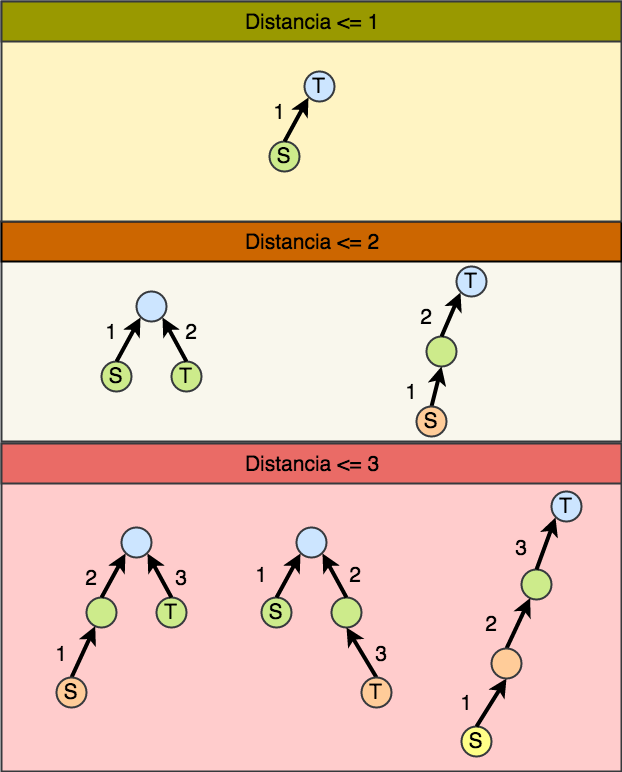
\includegraphics[width=0.5\textwidth]{distancias_semanticas}
\end{figure}

% Please add the following required packages to your document preamble:
% \usepackage{booktabs}
% \usepackage{multirow}
\begin{table}[htb]
\centering
\caption{Cubrimientos de servicios con distancias semánticas entre 1 y 3}
\label{cubrimiento_1y3}
\resizebox{\textwidth}{!}{%
\begin{tabular}{@{}lrrrrrrrr@{}}
\toprule
\multirow{2}{*}{Servicio} & \multicolumn{2}{l}{\begin{tabular}[c]{@{}l@{}}Cubrimientos con \\ Distancia Semántica \textless=3\end{tabular}} & \multicolumn{2}{l}{\begin{tabular}[c]{@{}l@{}}Cubrimientos con \\ Distancia Semántica \textless=2\end{tabular}} & \multicolumn{2}{l}{\begin{tabular}[c]{@{}l@{}}Cubrimientos con \\ Distancia Semántica \textless=1\end{tabular}} & \multicolumn{2}{l}{Cubrimientos exactos} \\ \cmidrule(l){2-9} 
 & Kaiser/Hiba & Hiba/Kaiser & Kaiser/Hiba & Hiba/Kaiser & Kaiser/Hiba & Hiba/Kaiser & Kaiser/Hiba & Hiba/Kaiser \\ \cmidrule(r){1-9}
Cardio & 0,475 & 0,947 & 0,320 & 0,890 & 0,211 & 0,782 & 0,104 & 0,457 \\
Oftalmo & 0,779 & 0,969 & 0,647 & 0,949 & 0,505 & 0,787 & 0,257 & 0,407 \\
Derma & 0,831 & 0,974 & 0,683 & 0,942 & 0,452 & 0,824 & 0,242 & 0,449 \\
Pedia & 0,85 & 0,973 & 0,769 & 0,940 & 0,594 & 0,857 & 0,305 & 0,560 \\
ENU & 0,492 & 0,979 & 0,319 & 0,944 & 0,174 & 0,811 & 0,075 & 0,403 \\
Onco & 0,582 & 0,879 & 0,433 & 0,623 & 0,307 & 0,252 & 0,073 & 0,173 \\
Psiqui & 0,572 & 0,904 & 0,476 & 0,813 & 0,384 & 0,627 & 0,227 & 0,303 \\
Orto & 0,726 & 0,986 & 0,586 & 0,963 & 0,402 & 0,860 & 0,179 & 0,420 \\
Neuro & 0,563 & 0,975 & 0,385 & 0,963 & 0,227 & 0,825 & 0,112 & 0,404 \\
Gineco & 0,597 & 0,936 & 0,443 & 0,904 & 0,284 & 0,743 & 0,119 & 0,326 \\ \bottomrule
\end{tabular}%
}
\end{table}

Como se muestra en la tabla \ref{cubrimiento_1y3}, hay una significativa mejora en los valores de cubrimiento, incluso con distancia \textless=2 todos alcanzan más de un 90\% de cubrimiento de conceptos del Kaiser por el HIBA, con excepción de Oncología. Esta mejora se explica porque el crecimiento del HIBA agrega hasta un nivel más de precisión, muchos conceptos son descendientes del mismo ancestro y al no ser tenido en cuenta porque no hay un \textit{match} exacto se descartan también todas esas ramas que crecen a lo ancho.

En el caso del cubrimiento de los conceptos de HIBA por el Kaiser, el cubrimiento también mejora pero sigue siendo muy pequeño, esto se debe a que el HIBA tiene no sólo más conceptos en los \textit{refsets} sino que se evidencia una mayor diversidad en ellos.
 
Por último, en la fase de implementación eliminé las que entraron en el criterio de exclusión y reemplacé las áreas jerárquicas con 29 servicios de atención de Snomed CT.


\subsubsection{Contexto: Nivel de asistencia}
Con el fin de encontrar conceptos que estén asociados a los niveles de asistencia apliqué los algoritmos agrupamiento \textit{leading vector}, \textit{label propagation} y \textit{multilevel}. Los valores de modularidad y número de grupos son similares en aplicando todos los algoritmos:
\begin{itemize}
\item \textit{Leading vector}, modularidad = \num{0.346} y número de grupos = 4
\item \textit{Label propagation}, modularidad = \num{0.393} y número de grupos = 5
\item \textit{Multilevel}, modularidad = \num{0.397} y número de grupos = 5
\end{itemize}

Según la tabla \ref{nivel_asistencia} se puede observar que en 4 niveles de asistencia (Ambulatorio, Guardia, Triage e Internación general) están el 97\% del total de los registros de la lista de problemas. De estos 4 niveles de asistencia, en el caso de Ambulatoria y Guardia hay una relación en la que por cada 10 registros hay 1 concepto de Snomed CT diferente asociado a la lista de problemas, Triage es la relación más baja ya que es 20:1 entre los registros y los conceptos de Snomed  CT, e Internación General es la más alta (10:2). Al aplicar los algoritmos de agrupamiento, se fusionaron los niveles de asistencia Internación general e Internación domiciliaria, con 3002 conceptos que representan su contexto, y se descarta el nivel de asistencia Episodio externo.

\begin{table}[htb]
\centering
\caption{Distribución de registros y conceptos por nivel de asistencia o ámbito }
\label{nivel_asistencia}
\begin{tabular}{@{}lrrr@{}}
\toprule
Nivel de Asistencia o ámbito & Registros & Diferentes Conceptos& Conceptos del grupo \\ \midrule
Ambulatorio & \num{771096} & \num{9543}& \num{6304} \\
Guardia & \num{603412} & \num{5759}& \num{2269} \\
Triage & \num{556166} & \num{2963}& \num{779} \\
Internación general & \num{267303} & \num{6322}& \num{3002} \\
Internación domiciliaria & \num{22297} & \num{1975} & \num{3002}\\
Episodio ambulatorio & \num{17947} & \num{1247}& \num{370} \\
Seguimiento domiciliario & \num{14537} & \num{1302} & \num{681}\\
Internación geriátrica & \num{204} & \num{115}& \num{101} \\
Episodio externo & \num{4} & \num{2} & \num{0}\\ \bottomrule
\end{tabular}
\end{table}


\subsubsection{Contexto: Grupo etario}
La distribución de los problemas registrados por edad en la figura \ref{fig:listaEdad} evidencia que los grupos etarios en los que más se consulta son 0-4 años, 25-34 años y mayores de 75 años.

Al aplicar los algoritmos de agrupamiento, obtengo resultados similares entre \textit{Leading vector} y \textit{multilevel}. \textit{Leading Vector} dividió el grafo en 5 grupos y obtuvo una modularidad de \num{0.171}, \textit{multilevel} dividió el grafo en 4 grupos y obtuvo una modularidad de \num{0.138}. En el caso del algoritmo \textit{label propagation} el valor de la modularidad es de 0, por lo tanto sus resultados son descartados.

Después de combinar los resultados de los algoritmos \textit{Leading vector} y \textit{multilevel}, para identificar los grupos que invariantemente se repitan en ambos resultados, se descarta el grupo etario de 5 a 14 años y fusionan los grupos etarios de 0 a 4, 15 a 24, 25 a 34 y 35 a 44 años. La tabla \ref{grupo_etario} contiene los tamaños finales de los grupos.

\begin{figure}[ht]
\caption{Distribución de todos los problema por edad de los pacientes}
\label{fig:listaEdad}
\centering
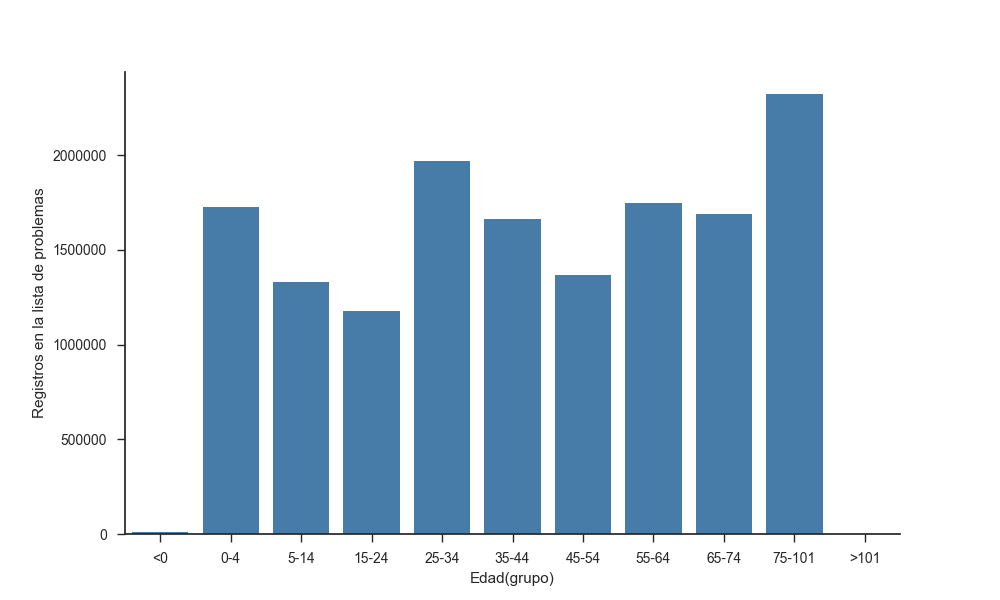
\includegraphics[width=\textwidth]{chart4}
\end{figure}

% Please add the following required packages to your document preamble:
% \usepackage{booktabs}
\begin{table}[htb]
\centering
\caption{Distribución de conceptos por grupo etario }
\label{grupo_etario}
\begin{tabular}{@{}lrr@{}}
\toprule
Grupo Etario & Diferentes Conceptos & Conceptos del grupo \\ \midrule
0-4 & \num{15264} & \num{12532} \\
5-14 & \num{24837} & \num{0} \\
15-24 & \num{29548} & \num{12532} \\
25-34 & \num{35419} & \num{12532} \\
35-44 & \num{33165} & \num{12532} \\
45-54 & \num{32644} & \num{6731} \\
55-64 & \num{35733} & \num{5073} \\
65-74 & \num{35772} & \num{5165} \\
75-101 & \num{37625} & \num{4292} \\ \bottomrule
\end{tabular}
\end{table}

\section{Discusión}
El objetivo de este capítulo era el análisis descriptivo de los datos y de los procesos de limpieza que apliqué para obtener un conjunto de datos consistente con el que realizar los experimentos de graphmining en el siguiente capítulo.

En la primera sección abordé la comprensión de los datos de la lista de problemas. Este análisis me permitió identificar outliers y datos de error al momento de la carga, revisando la distribución desde diferentes dimensiones: tiempo, individuos, conceptos y contextos: 

(a) en el caso del tiempo sólo son válidos los registros con fecha de carga desde el año 1998 hasta el tiempo presente, dado que este ha sido el lapso en el que ha estado activa la HCE; 

(b) desde el punto de vista de los individuos  el 34.1\% tiene sólo un problema, estos registros también se descartan porque carecen de co-ocurrencia con otros problemas; 

(c) en la dimensión de los conceptos, el 20\% de los registros pertenecen a 12 conceptos y sus variantes lexicográficas, estos problemas tendrán poca capacidad predictiva dado que se relacionarán con un número grande de conceptos. El uso de los conceptos presenta una distribución de cola larga, esto es consistente por lo reportado por Fung et. al.\cite{Fung2015AnCT} donde haciendo una comparación del uso de la lista de problemas de ocho instituciones, encontró que el 95\% del uso corresponde a sólo el 22.8\% de términos únicos;

(d) Los contextos analizados fueron el área jerárquica, nivel de asistencia y grupo etario, cada uno de estos contextos tiene sus particularidades.

El HIBA tiene 601 áreas jerárquicas con diferentes niveles de agregación, algunas de esas áreas corresponden a funciones administrativas. El experimento 1 permitió excluir las áreas administrativas y mapear las restantes a  44 servicios de SNOMED CT, facilitando así la interoperabilidad con otros centros médicos. 

El experimento 2 mostró que algunos de los servicios se solapan entre sí, ya que significativamente un clasificador no puede diferenciar cuándo los conceptos pertenecen a un servicio u otro, entre los servicios con F1 score más bajos tengo: servicio de anestesia (0,048), servicio audiológico (0,000), servicio de colposcopia (0,000), servicio de internación domiciliaria (0,131), servicio de patología (0,000) y servicio de psicología (0,000). Estos servicios fueron fusionados con los que más presentaban solapamiento en la matriz de confusión.

Los servicios con mejor F1 score son: servicio de cardiología pediátrica (0,871), servicio de fisioterapia (0,993), servicio de ginecoobstetricia (0,877), servicio de oftalmología adultos (0,938), servicio de psiquiatría (0,827), servicio de psiquiatria pediatrica(0,945) y  servicio de traumatología (0,821). Estos valores muestran que los conceptos diferencian bien estos servicios, y que no deberían ser fusionados aunque uno sea padre del otro como el caso de  servicio de psiquiatría y servicio de psiquiatria pediatrica.

Como resultado de esos experimentos obtuve 29 servicios finales, para evaluar el cubrimiento de los \textit{refsets}, use como referencia los donados por Kaiser Permanente a Snomed CT, en ellos encontré 10 \textit{refsets} de Kaiser Permanente que eran afines a 16 de los 29 servicios finales. Los resultados obtenidos muestran que la mayoría de los servicios tienen una cobertura entre 0,30 y 0,45, los que se ubican con mejor cobertura son pediatría (0,56), cardiología(0,46) y dermatología (0,45); y el de peor cobertura es oncología (0,07), este es el único caso en el que el \textit{refset} creado por el HIBA es de menor tamaño al de referencia, en todos los otros casos el tamaño de los \textit{refsets} del HIBA es superior en tamaño a los de referencia. 

Los niveles de precisión entre los dos conjuntos de datos hace compleja la tarea de comparación, cuando cuento los conceptos que se encuentran en el \textit{refset} de referencia, no sólo debo de tener en cuenta los mapeos directos o las relaciones is\_a exactas, porque pierdo a los conceptos que tienen mayor precisión. Por lo tanto, contrasté estos resultados con la cobertura calculada con diferentes distancias semánticas, encontrando que hay una significativa mejora en los valores de cubrimiento, incluso con distancia \textless= 2 la mayoría de los servicios alcanzan más de un 90\% de cubrimiento de conceptos del Kaiser.

Un trabajo similar reportado por Nova Scotia\cite{nova}, en el que desarrollan sus propios \textit{refsets} de especialidades, obtiene coberturas inferiores a las reportadas en esta tesis, incluso sin el cálculo de distancias semánticas (ver tabla \ref{coverage_scotia}). 

\begin{table}
 \caption{Comparación de la cobertura de las especialidades del HIBA vs Nova Scotia }
  \label{coverage_scotia}
  \resizebox{\textwidth}{!}{%
  \begin{tabular}{lcccccc} \hline
 \small
& \multicolumn{3} {c}{ Nova Scotia} & \multicolumn{3} {c}{HIBA} \\ \hline
Servicio& \# Refset & \# Kaiser & Cobertura &\# Refset & \# Kaiser  & Cobertura  \\ \hline
Cardiología&886&653 &0,18&9182&880  &0,46 \\
Dermatoloía&638&691    &0,16&11622&2757     &0,45 \\
Hematología*&714&330   &0,13&721&4086    &0,17\\
Enfermedades infecciosas&2,202&1101   &0,08&-&-&  \\
Oftamología&1,327&413&    0,34&4188&3285     &0.41\\
Cirugía ortopédica&1,306&167&   0,10&22555&1089    &0,25\\
Otoloaringología&1,344&641    &0,29&-&-&  \\
Pediatría&3,699&2181    &0,34&17325&3793     &0,56\\
Medicina respiratoria&114&511   &0,08&-&-&\\\hline

\end{tabular}
 %
}
\end{table}

En el nivel de asistencia hay desbalanceo entre los grupos. Los grupos más grandes son el nivel de asistencia ambulatorio (6304 conceptos), las internaciones que se fusionaron en una sola (3002), y la guardia (2269). Aunque el nivel de asistencia de Triage sea el tercero en cantidad de registros, el número de conceptos en su grupo es muy pequeño, lo que indica la baja diversidad de conceptos seleccionados en este nivel de asistencia. 

Los grupos etarios que más registran problemas son entre los 0-4 años, 25 y 34 años y mayores de 75 años, los registros con edades menores a 0 o mayores a 101 fueron descartadas por interpretarse como errores del sistema o casos de prueba. Utilizando los algoritmos de agrupación se fusionaron los grupos etarios entre los 0 y 44 años. Según estos algoritmos, los problemas que existen en estos grupos no tienen diferencias significativas. Al mismo tiempo, descarté el grupo etario entre 5 y 14 años, ya que los problemas no se agruparon en un grupo consistente.

\section{Conclusión}
En este capítulo he presentado las decisiones en la extracción, transformación y limpieza de la lista de problemas, para definir el conjunto de datos que será utilizado en los experimentos de graphmining. 

La transformación más compleja fue la de la definición del contexto de los 29 servicios de atención a partir de las 901 áreas jerárquicas. Si bien agrupar los conceptos por contexto es necesario para facilitar el uso significativo de la SNOMED CT, son escasos los ejemplos sobre metodologías o \textit{refsets} públicos que puedan ser usados como referencia.

En este capítulo usé técnicas de agrupamiento y aprendizaje supervisado para definir qué servicios, niveles asistenciales y grupos etarios pueden ser diferenciables de los demás a partir de sus conceptos. En el caso de los servicios, Una vez fueron definidos evalué su cubrimiento con respecto a los \textit{refsets} de referencia de kaiser permanente, aunque en la mayoría de los casos da un cubrimiento exacto superior al 40\%, si se utilizan las distancias semánticas estos cubrimientos se incrementan significativamente.

Con respecto a las distancias semánticas, este trabajo no tiene en cuenta el nivel de granularidad de los conceptos que se están comparando, por lo tanto un par de conceptos que estén muy arriba en la jerarquía y sean muy generales tienen igual distancia que dos conceptos que estén muy abajo y sean muy específicos. Sin embargo, en la práctica entre más precisos sean los conceptos que tienen similitud, se puede confiar más en que realmente tienen un significado similar.
